% ==============================================================================
% CAPÍTULO 3: DISEÑO GEOMÉTRICO Y PERFILES DE CAMPO ELÉCTRICO
% ==============================================================================
\chapter{Diseño Geométrico y Perfiles de Campo Eléctrico}

\section{Evolución Geométrico-Cinemática de las Celdas Síncronas}
El diseño de la cavidad resonante tipo Álvarez para la aceleración de protones se fundamenta en la estricta preservación de la condición de sincronismo relativista celda a celda. Para una frecuencia de radiofrecuencia nominal $f_{\text{RF}} = 352.2\text{ MHz}$, la longitud de onda en el vacío del campo electromagnético es $\lambda = c / f_{\text{RF}} \approx 0.8512\text{ m}$.

Dado que la ganancia de energía cinética por celda para la partícula síncrona es constante ($\Delta T = q V_{\text{gap}} \cos\phi_s = 1.0\text{ MV} \cdot \cos(-30^\circ) \approx 0.866025\text{ MeV}$), la energía acumulada al finalizar la celda $n$ aumenta de forma estrictamente lineal de acuerdo con:
\begin{equation}
T_n = T_0 + n \cdot q V_{\text{gap}} \cos(\phi_s)
\end{equation}

Como consecuencia del incremento sostenido en la energía cinética de $T_0 = 3.0\text{ MeV}$ a $T_{55} = 50.631\text{ MeV}$, el factor relativista de velocidad $\beta_n$ pasa de $0.0905$ en la primera celda a $0.3159$ en la celda final. Por lo tanto, las celdas síncronas experimentan una expansión longitudinal continua calculada mediante $L_n = \beta_n \lambda$, pasando de $L_1 = 0.077033\text{ m}$ ($7.70\text{ cm}$) a $L_{55} = 0.268874\text{ m}$ ($26.89\text{ cm}$).

\begin{figure}[H]
    \centering
    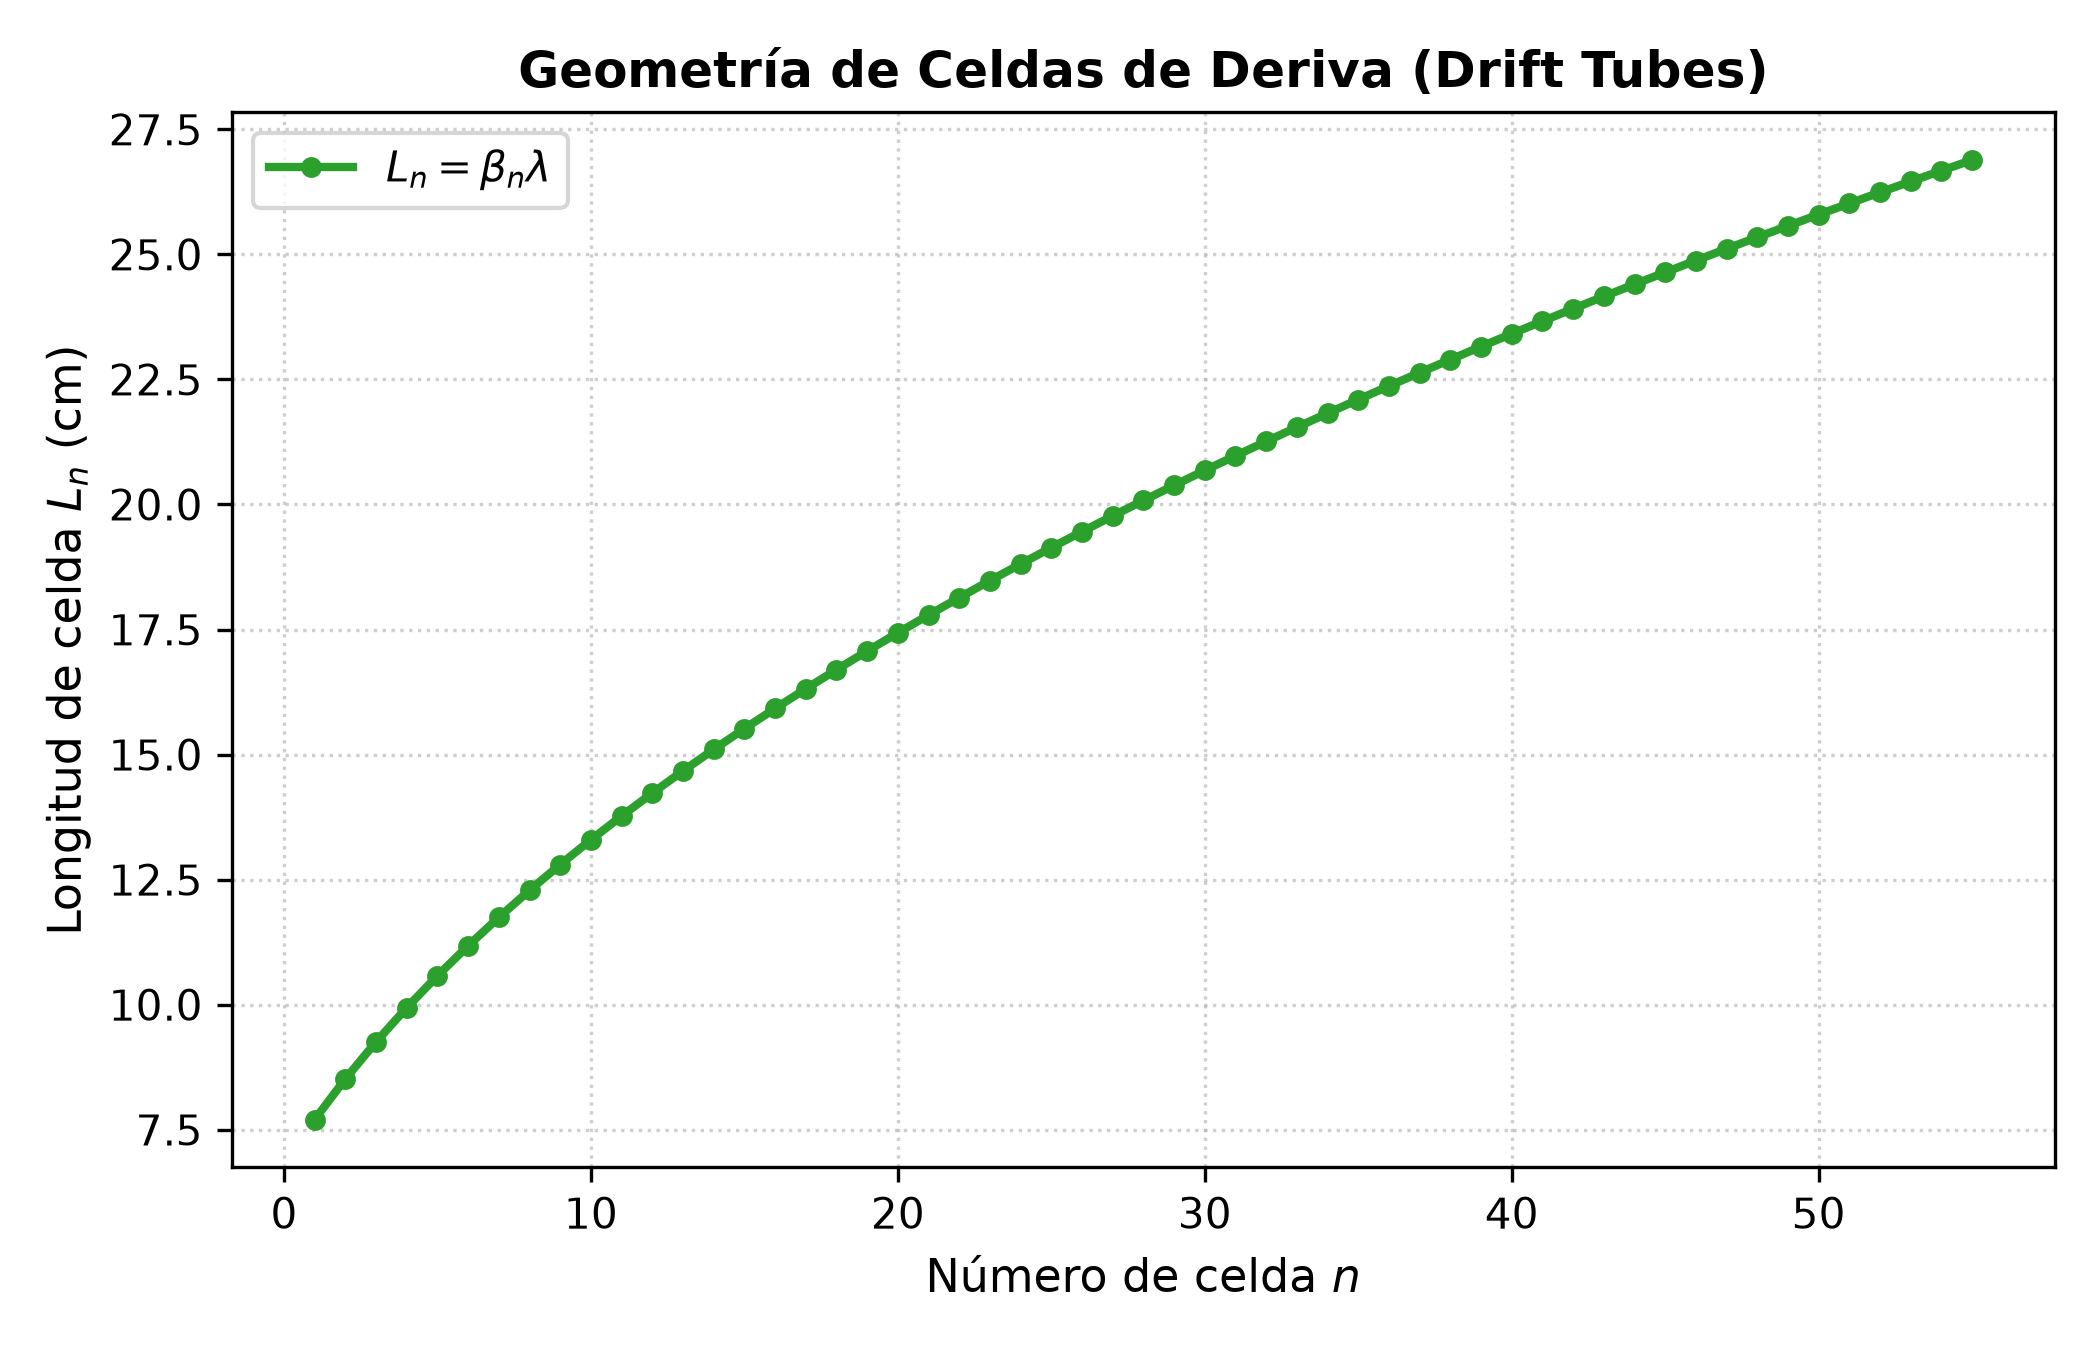
\includegraphics[width=0.85\textwidth]{figuras/fig01_diseno.png}
    \caption{Perfil geométrico del incremento de longitud de celdas síncronas $L_n = \beta_n \lambda$ a lo largo de las 55 celdas del LINAC Álvarez.}
    \label{fig:diseno_celdas}
\end{figure}

En la Figura \ref{fig:diseno_celdas} se aprecia la curvatura cóncava inicial en la longitud de las celdas, reflejando el rápido cambio cinemático en el régimen no relativista ($\beta \propto \sqrt{T}$ para $T \ll m_0 c^2$), seguida de una transición gradualmente lineal a medida que la inercia relativista limita la aceleración efectiva.

\section{Distribución del Campo Eléctrico y Gradientes de Aceleración}
Un aspecto físico central en el análisis de cavidades resonantes tipo Álvarez es la distinción formal entre el gradiente pico nominal $E_{0,n}$ y el gradiente de aceleración síncrono efectivo $E_{\text{acc},n}$. Ambas magnitudes se definen como promedios espaciales sobre la longitud total de la celda $n$:

\begin{equation}
E_{0,n} = \frac{q V_{\text{gap}}}{L_n} = \frac{1.0\text{ MV}}{L_n}
\end{equation}

\begin{equation}
E_{\text{acc},n} = \frac{\Delta T}{L_n} = \frac{q V_{\text{gap}} \cos(\phi_s)}{L_n} = E_{0,n} \cos(\phi_s)
\end{equation}

Dado que la tensión en el hueco de aceleración ($V_{\text{gap}} = 1.0\text{ MV}$) se mantiene constante a lo largo de toda la cavidad, la densidad de aceleración por unidad de longitud ($\text{MV/m}$) disminuye de forma inversamente proporcional a la longitud de la celda $L_n$.

\begin{figure}[H]
    \centering
    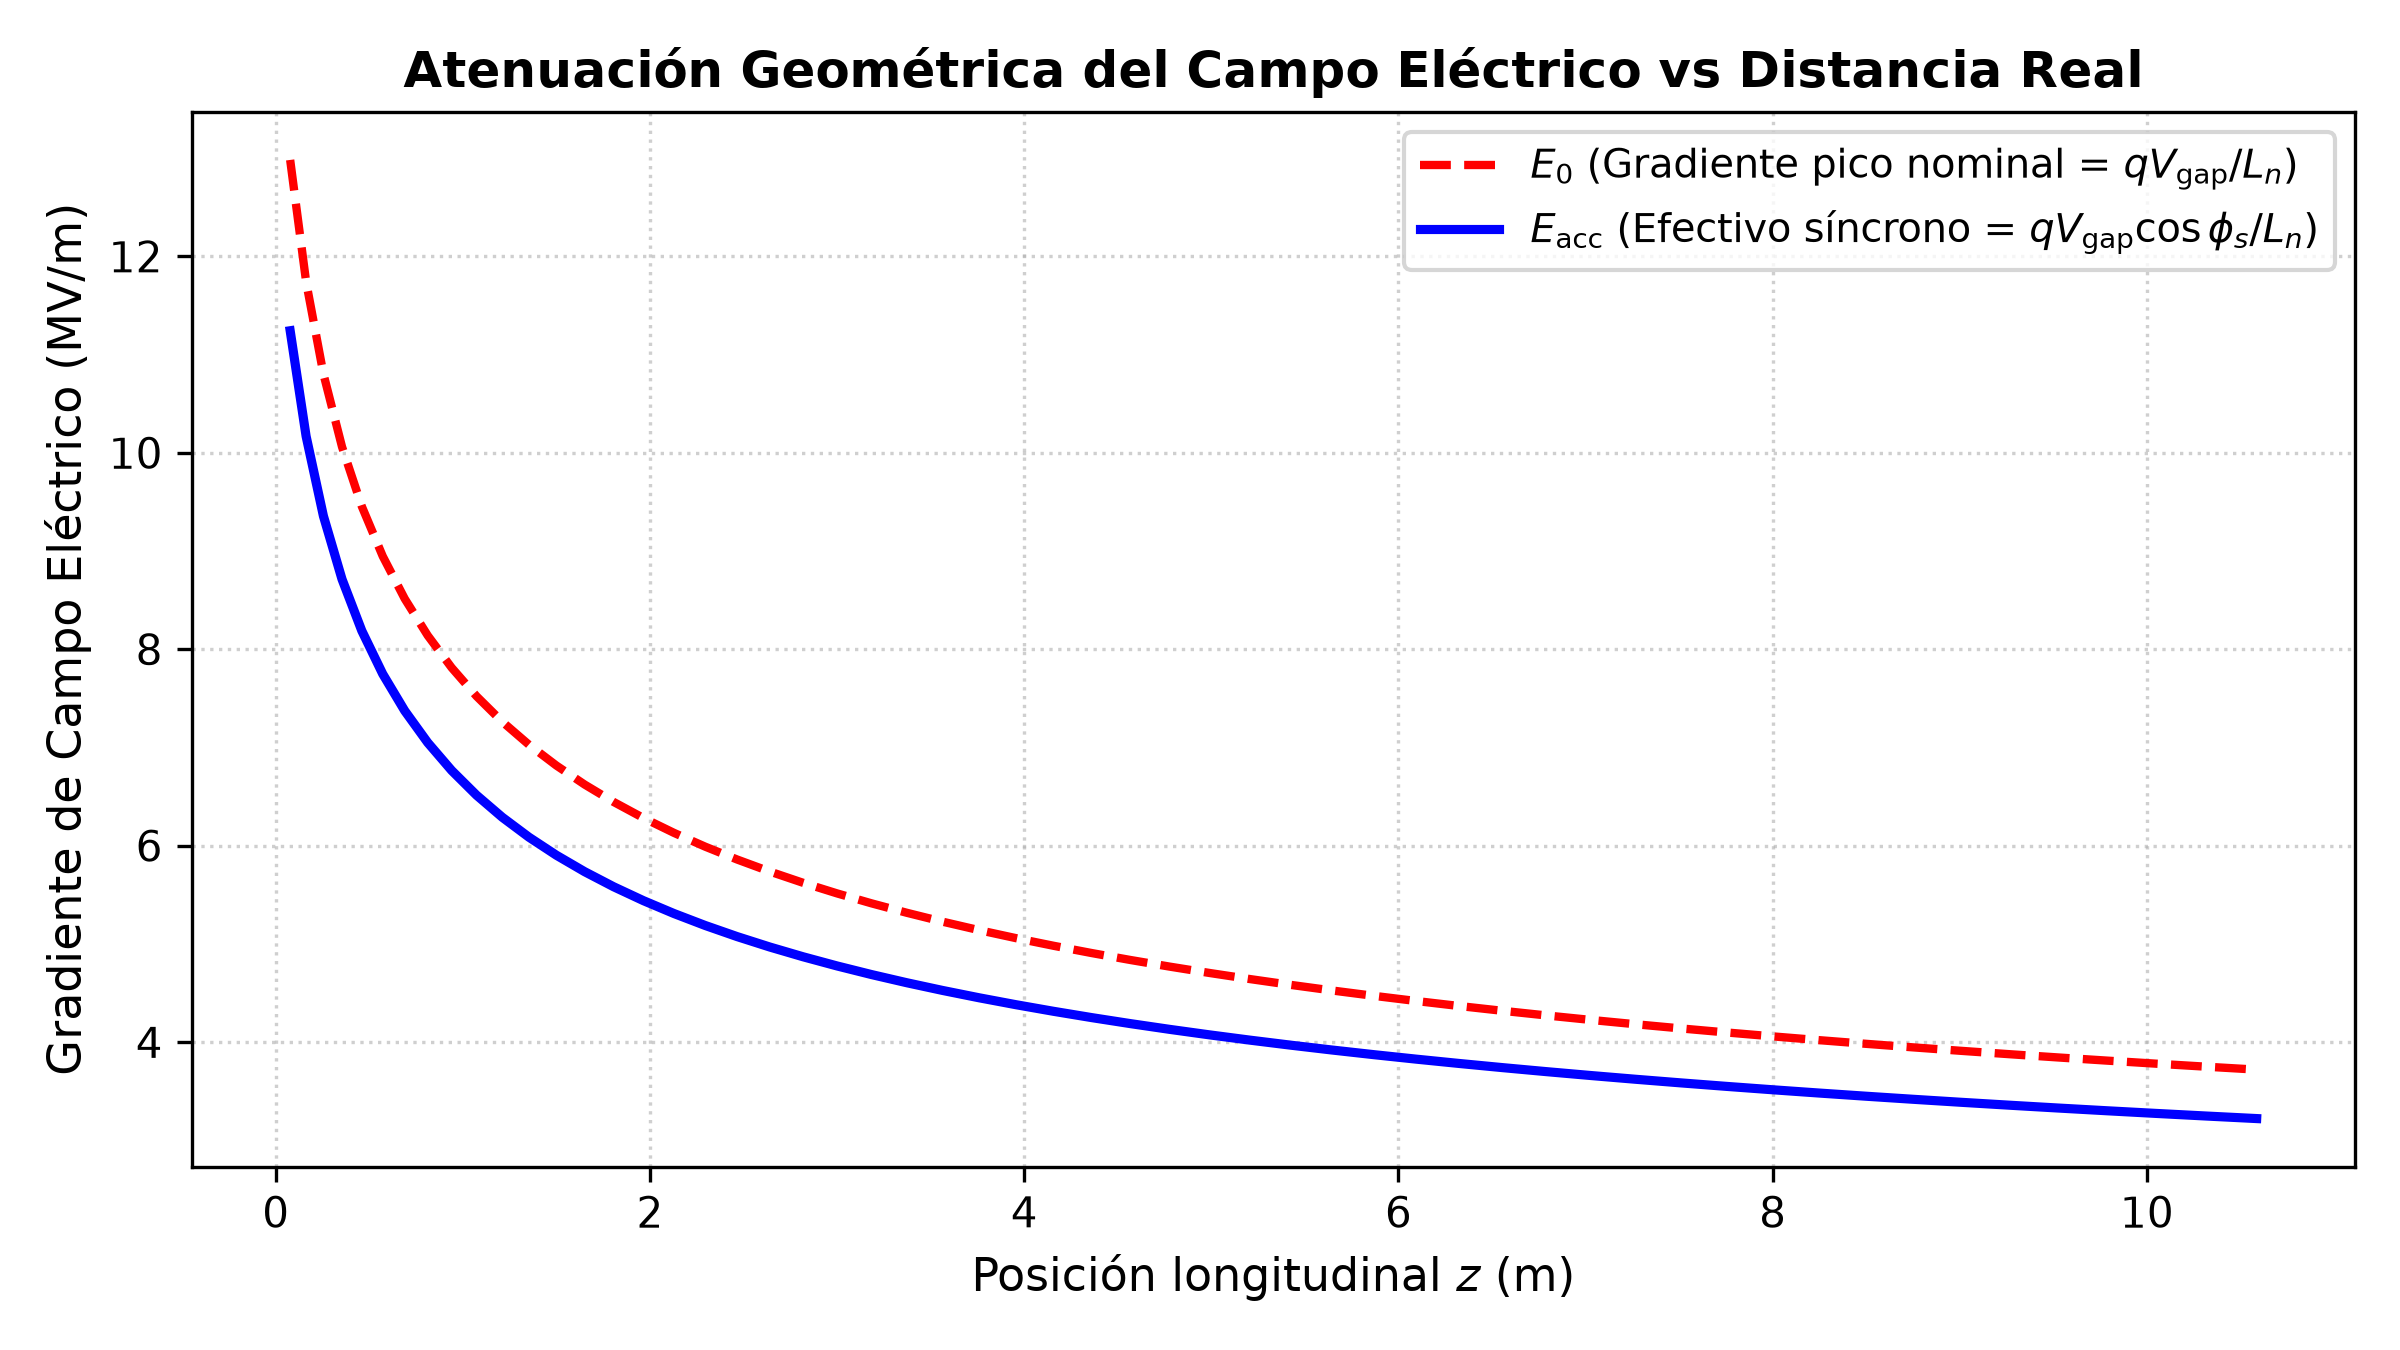
\includegraphics[width=0.88\textwidth]{figuras/fig06_perfil_campos.png}
    \caption{Perfil de atenuación geométrica del gradiente de campo eléctrico pico nominal ($E_0$) y del gradiente de aceleración efectivo síncrono ($E_{\text{acc}}$) en función de la posición longitudinal real $z$ (m).}
    \label{fig:perfil_campos}
\end{figure}

Como se ilustra en la Figura \ref{fig:perfil_campos}:
\begin{itemize}
    \item En la región de inyección ($z = 0.077\text{ m}$, Celda 1), el acelerador requiere un gradiente efectivo elevado de $E_{\text{acc},1} = 11.242\text{ MV/m}$ ($E_{0,1} = 12.981\text{ MV/m}$) debido a la brevedad del recorrido de la celda ($7.70\text{ cm}$).
    \item En la región de extracción ($z = 10.587\text{ m}$, Celda 55), la distribución de la misma ganancia energética ($0.866\text{ MeV}$) sobre una distancia mayor ($26.89\text{ cm}$) diluye el gradiente efectivo a $E_{\text{acc},55} = 3.221\text{ MV/m}$ ($E_{0,55} = 3.719\text{ MV/m}$).
\end{itemize}

\section{Perfil Cinemático Combinado y Resumen Geométrico}
La acumulación espacial de las longitudes de las 55 celdas determina una longitud total de la cavidad resonante de $z_{\text{total}} = 10.5867\text{ m} \approx 10.59\text{ m}$.

En la Figura \ref{fig:perfil_cinematico} se presenta la evolución simultánea de la velocidad relativa $\beta = v/c$ (eje izquierdo) y la energía cinética $T$ (eje derecho) respecto a la coordenada axial continua $z$.

\begin{figure}[H]
    \centering
    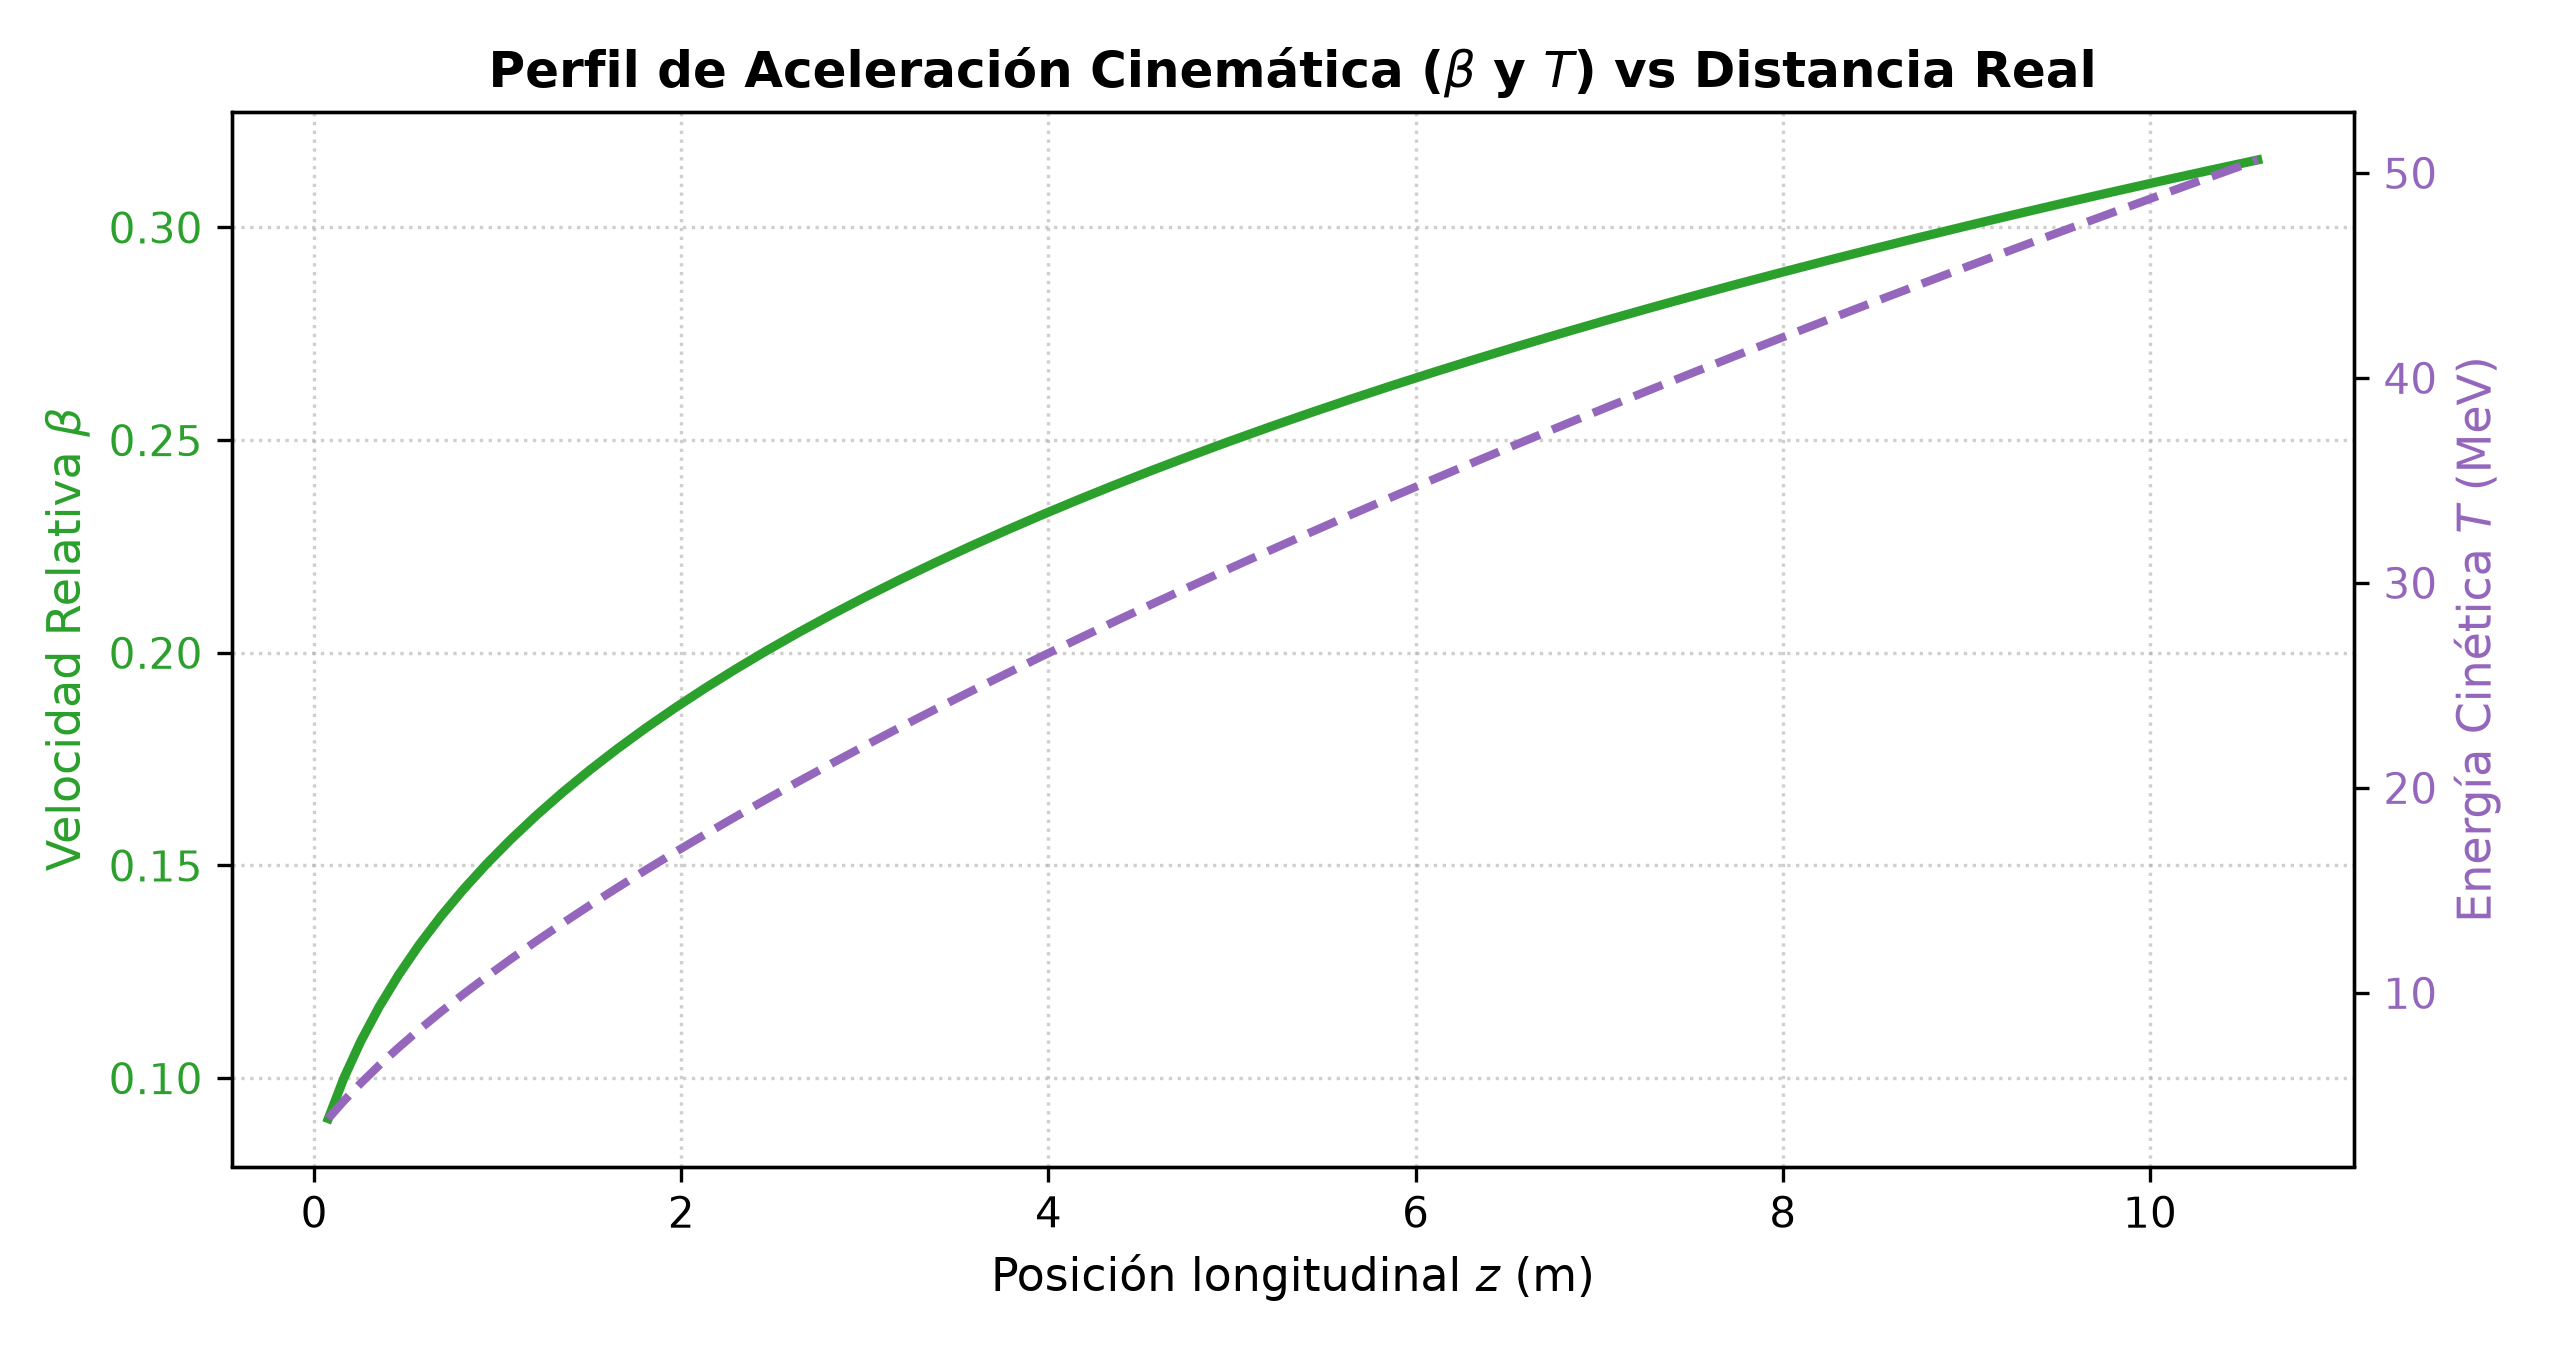
\includegraphics[width=0.88\textwidth]{figuras/fig08_perfil_cinematico.png}
    \caption{Perfil combinado de aceleración cinemática: evolución de la velocidad adimensional $\beta$ y la energía cinética síncrona $T$ (MeV) en función de la distancia longitudinal $z$.}
    \label{fig:perfil_cinematico}
\end{figure}

\begin{table}[H]
    \centering
    \caption{Parámetros cinemáticos, geométricos y de campo eléctrico para celdas representativas del LINAC Álvarez de 55 celdas.}
    \label{tab:diseno_resumen}
    \vspace{0.2cm}
    \small
    \setlength{\tabcolsep}{4pt}
    \resizebox{\textwidth}{!}{%
    \begin{tabular}{cccccccc}
        \toprule
        \textbf{Celda $n$} & $L_n$ (m) & $z_n$ (m) & $T_{\text{sync}}$ (MeV) & $\beta$ & $\gamma$ & $E_{\text{acc}}$ (MV/m) & $E_0$ (MV/m) \\
        \midrule
        1  & 0.077033 & 0.077033 & 3.866 & 0.0905 & 1.0041 & 11.242 & 12.981 \\
        10 & 0.132959 & 1.118991 & 11.660 & 0.1562 & 1.0124 & 6.513  & 7.521  \\
        20 & 0.174780 & 2.664402 & 20.321 & 0.2053 & 1.0217 & 4.955  & 5.721  \\
        30 & 0.207865 & 4.582845 & 28.981 & 0.2442 & 1.0309 & 4.166  & 4.811  \\
        40 & 0.235955 & 6.806297 & 37.641 & 0.2772 & 1.0401 & 3.670  & 4.238  \\
        50 & 0.260191 & 9.294488 & 46.301 & 0.3057 & 1.0493 & 3.328  & 3.843  \\
        55 & 0.268874 & 10.586696 & 50.631 & 0.3159 & 1.0540 & 3.221  & 3.719  \\
        \bottomrule
    \end{tabular}%
    }
\end{table}